\documentclass[]{elsarticle} %review=doublespace preprint=single 5p=2 column
%%% Begin My package additions %%%%%%%%%%%%%%%%%%%
\usepackage[hyphens]{url}



\usepackage{lineno} % add
\providecommand{\tightlist}{%
  \setlength{\itemsep}{0pt}\setlength{\parskip}{0pt}}

\usepackage{graphicx}
\usepackage{booktabs} % book-quality tables
%%%%%%%%%%%%%%%% end my additions to header

\usepackage[T1]{fontenc}
\usepackage{lmodern}
\usepackage{amssymb,amsmath}
\usepackage{ifxetex,ifluatex}
\usepackage{fixltx2e} % provides \textsubscript
% use upquote if available, for straight quotes in verbatim environments
\IfFileExists{upquote.sty}{\usepackage{upquote}}{}
\ifnum 0\ifxetex 1\fi\ifluatex 1\fi=0 % if pdftex
  \usepackage[utf8]{inputenc}
\else % if luatex or xelatex
  \usepackage{fontspec}
  \ifxetex
    \usepackage{xltxtra,xunicode}
  \fi
  \defaultfontfeatures{Mapping=tex-text,Scale=MatchLowercase}
  \newcommand{\euro}{€}
\fi
% use microtype if available
\IfFileExists{microtype.sty}{\usepackage{microtype}}{}
\bibliographystyle{elsarticle-harv}
\ifxetex
  \usepackage[setpagesize=false, % page size defined by xetex
              unicode=false, % unicode breaks when used with xetex
              xetex]{hyperref}
\else
  \usepackage[unicode=true]{hyperref}
\fi
\hypersetup{breaklinks=true,
            bookmarks=true,
            pdfauthor={},
            pdftitle={Statistical Inference for inter-arrival times of extreme events in bursty time series},
            colorlinks=false,
            urlcolor=blue,
            linkcolor=magenta,
            pdfborder={0 0 0}}
\urlstyle{same}  % don't use monospace font for urls

\setcounter{secnumdepth}{5}
% Pandoc toggle for numbering sections (defaults to be off)
% Pandoc header



\begin{document}
\begin{frontmatter}

  \title{Statistical Inference for inter-arrival times of extreme events in
bursty time series}
    \author[a]{Katharina Hees}
   \ead{hees@statistik.tu-dortmund.de} 
  
    \author[b]{Smarak Nayak}
   \ead{smarak.nayak@nab.com.au} 
  
    \author[c]{Peter Straka}
   \ead{p.straka@unsw.edu.au} 
  
      \address[a]{Department of Statistics, TU Dortmund University, Dortmund, Germany}
    \address[b]{National Australia Bank, Melbourne, Australia}
    \address[c]{School of Mathematics and Statistics, UNSW, Sydney, Australia}
  
  \begin{abstract}
  In many complex systems studied in statistical physics, inter-arrival
  times between events such as solar flares, trades and neuron voltages
  follow a heavy-tailed distribution. The set of event times is
  fractal-like, being dense in some time windows and empty in others, a
  phenomenon which has been dubbed ``bursty''.
  
  This article proposes a new model for the \emph{inter-exceedance times}
  of events above high thresholds; the threshold exceedances itself are
  modeled via the standard Peaks-Over-Threshold (POT) method. For high
  thresholds and infinite-mean waiting times, we show that the times
  between threshold crossings are Mittag-Leffler distributed, and thus
  form a ``fractional Poisson Process'' which generalizes the standard
  Poisson Process of threshold exceedances. We provide graphical means of
  estimating model parameters and assessing model fit. Along the way, we
  apply our inference method to a real-world bursty time series, and show
  how the memory of the Mittag-Leffler distribution affects the predictive
  distribution for the time until the next extreme event.
  \end{abstract}
   \begin{keyword} heavy tails renewal process extreme value theory peaks over threshold\end{keyword}
 \end{frontmatter}

\hypertarget{introduction}{%
\section{Introduction}\label{introduction}}

Time series displaying temporally inhomogeneous behaviour in terms of
the occurrence of events have received strong interest in the recent
statistical physics literature (Barabási 2005; Oliveira and Barabási
2005; Vasquez et al. 2006; Vazquez et al. 2007; Omi and Shinomoto 2011;
Min, Goh, and Vazquez 2011; Karsai et al. 2011; Bagrow and Brockmann
2013). They have been observed in the context of earthquakes, sunspots,
neuronal activity and human communication (see Karsai et al. 2012;
Vajna, Tóth, and Kertész 2013; Meerschaert and Stoev 2008 for a list of
references). Such time series exhibit high activity in some `bursty'
intervals, which alternate with other, quiet intervals. Although several
mechanisms are plausible explanations for bursty behaviour (most
prominently self-exciting point process by Hawkes (1971)), there seems
to be one salient feature which very typically indicates the departure
from temporal homogeneity: a heavy-tailed distribution of waiting times
(Vasquez et al. 2006; Karsai et al. 2012; Vajna, Tóth, and Kertész
2013). As we show below in simulations, a simple renewal process with
heavy-tailed waiting times can capture this type of dynamics. For many
systems, the renewal property is appropriate; a simple test of the
absence of correlations in a succession of waiting times can be
undertaken by randomly reshuffling the waiting times (Karsai et al.
2012).

Often a magnitude, or mark can be assigned to each event in the renewal
process, such as for earthquakes, solar flares or neuron voltages. The
Peaks-Over-Threshold model (POT, see e.g.~Coles 2001) applies a
threshold to the magnitudes, and fits a Generalized Pareto distribution
to the threshold exceedances. A commonly made assumption in POT models
is that times between events are either fixed or light-tailed, and this
entails that the threshold crossing times form a Poisson process (``On
the Exceedance Point Process for a Stationary Sequence'' 1988). Then as
one increases the threshold and thus decreases the threshold crossing
probability \(p\), the Poisson process is rarefied, i.e.~its intensity
decreases \emph{linearly} with \(p\) (see e.g.~Beirlant et al. 2006).

As will be shown below, in the heavy-tailed waiting time scenario
threshold crossing times form a \emph{fractional Poisson process}
(Laskin 2003; Meerschaert, Nane, and Vellaisamy 2011), which is a
renewal process with Mittag-Leffler distributed waiting times. The
family of Mittag-Leffler distributions nests the exponential
distribution (Haubold, Mathai, and Saxena 2011), and hence the
fractional Poisson process generalizes the standard Poisson process.
Again as the threshold size increases and the threshold crossing
probability \(p\) decreases, the fractional Poisson process is rarefied:
The scale parameter of the Mittag-Leffler inter-arrival times of
threshold crossing times increases, but \emph{superlinearly}; see the
Theorem below.

Maxima of events which occur according to a renewal process with
heavy-tailed waiting times have been studied under the names
``Continuous Time Random Maxima process'' (CTRM) (Benson, Schumer, and
Meerschaert 2007; Meerschaert and Stoev 2008; Hees and Scheffler 2018b,
2018a), ``Max-Renewal process'' (Silvestrov 2002; Silvestrov and Teugels
2004; Basrak and Špoljarić 2015), and ``Shock process'' (Esary and
Marshall 1973; Shanthikumar and Sumita 1983, 1984, 1985; Anderson 1987;
Gut and Hüsler 1999). The existing literature focuses on probabilistic
results surrounding these models. In this work, however, we introduce a
method of inference for this type of model, which is seemingly not
available in the literature.

We review the marked renewal process in Section 2, and derive a scaling
limit theorem for inter-exceedance times in Section 3. We give a
statistical procedure to estimate model parameters via stability plots
in Section 5, but to set the stage we first discuss inference for the
Mittag-Leffler distribution in Section 4. A simulation study of the
effectiveness of our statistical procedure is given in Section 6. In
Section 7 we apply our method to a real data set. In Section 8, we
discuss the memory property of the Mittag-Leffler distribution, and how
it affects the predictive distribution for the time until the next
threshold crossing event. Finally we close with a discussion and
conclusion in Section 9. For all statistical computations we have used R
(R Core Team 2018). All code and data used for the analysis in this
article has been organized into an R package \texttt{CTRE}
(\url{https://github.com/strakaps/CTRE}). The source code for the
figures generated in this manuscript is available online at
\url{https://github.com/strakaps/bursty-POT}.

\hypertarget{continuous-time-random-exceedances-ctre}{%
\section{Continuous Time Random Exceedances
(CTRE)}\label{continuous-time-random-exceedances-ctre}}

As a model for extreme observations, we use a Marked Renewal Process
(MRP):

\begin{description}
\item[\textbf{Definition (MRP):}]
Let \((W,J), (W_1, J_1), (W_2, J_2), \ldots\) be i.i.d. pairs of random
variables, where the \(W_k > 0\) are interpreted as the \emph{waiting
times} and \(J_k \in [x_L, x_R]\) as the \emph{event magnitudes}
(\(x_L \in [-\infty, +\infty), x_R \in (-\infty, +\infty]\)). If \(W\)
and \(J\) are independent, the Marked Renewal Process is said to be
\emph{uncoupled}.
\end{description}

We assume that the \(k\)-th magnitude \(J_k\) occurs at time
\(T_k = W_1 + \ldots + W_k\). Based on an MRP, we define the Continuous
Time Random Exceedance model (CTRE) as follows:

\begin{description}
\item[\textbf{Definition (CTRE):}]
Given a threshold \(\ell \in (x_L, x_R)\), consider the stopping time
\[\tau(\ell) := \min\{k: J_k > \ell\},\quad \ell \in (x_L, x_R).\]
Define the pair of random variables \((X(\ell), T(\ell))\) via
\[X(\ell) = J_{\tau(\ell)} - \ell, \quad 
T(\ell) = \sum_{k=1}^{\tau(\ell)} W_k.\] By restarting the MRP at
\(\tau(\ell)\), inductively define the two i.i.d. sequences
\(T(\ell,n)\) and \(X(\ell, n)\), \(n \in \mathbb N\), called the
``inter-arrival times'' and the ``exceedances'', respectively. The pair
sequence \((T(\ell, n), W(\ell, n))_{n \in \mathbb N}\) is called a
Continuous Time Random Exceedance model (CTRE). If the underlying MRP is
uncoupled, then the CTRE is also called uncoupled.
\end{description}

\begin{figure}

{\centering 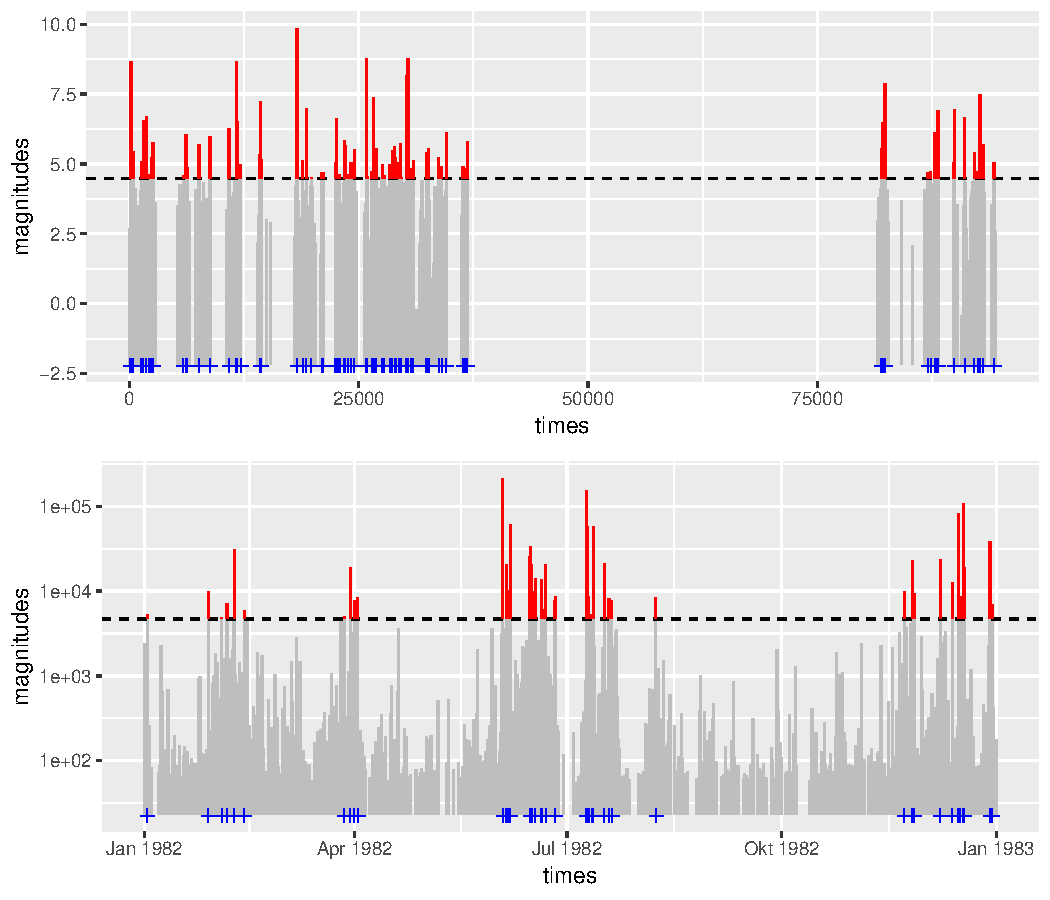
\includegraphics[width=0.7\linewidth]{article_springer_files/figure-latex/thresholdedBursty-1} 

}

\caption{\label{fig:thresholdedBursty} Exceedances (red) and times until Exceedance (durations between blue crosses) for a given threshold $\ell$ (dashed line). Upper picture: Simulated data with stable distributed waiting times. Lower picture: Solar flares during 1982.}\label{fig:thresholdedBursty}
\end{figure}

In this article, we restrict ourselves to the uncoupled case, where
\(W\) and \(J\) are independent. Then the two sequences
\(X(\ell, n)_{n \in \mathbb N}\) and \(T(\ell, n)_{n \in \mathbb N}\)
are independent as well. To see why, note that \(X(\ell)\) is, in
distribution, simply equal to \(J | J > \ell\), independent of any
waiting time \(W_k\).\\
Figure \ref{fig:thresholdedBursty} shows a simulated dataset in the top
panel, where \(W\) has a stable distribution with tail parameter
\(\beta =\) 0.8 (and skewness \(1\) and location \(0\)), and where \(J\)
is from a standard Gumbel distribution. In the bottom panel, we plot a
time series of solar flare intensities derived from a NASA dataset
(Dennis et al. 1991) which we will later examine more closely (see
Section 7). Clearly, the simulated data exhibit long intervals
\emph{without any} events, whereas in the real-world dataset events
appear continuously. The threshold exceedances, however, appear to have
visually similar statistical behaviour in both models. Observations
below a threshold are commonly discarded in Extreme Value Theory (POT
approach); likewise, the CTRE model interprets these observations as
noise and discards them.

\hypertarget{sec:scaling}{%
\section{Scaling limit of Exceedance Times}\label{sec:scaling}}

In this section we state and prove the key theorem, see below. For an
accessible introduction to regular variation and stable limit theorems,
we recommend the book by Mark M Meerschaert and Sikorskii (2012).

\begin{description}
\item[\textbf{Theorem:}]
Let the waiting times \(J_k\) be in the domain of attraction of a
positively skewed sum-stable law with stability parameter
\(0 < \beta < 1\); more precisely, \begin{align} \label{eq:stability}
\frac{W_1 + \ldots + W_n}{b(n)} \overset{d}{\longrightarrow} D, 
\quad n \to \infty
\end{align} for a function \(b(n)\) which is regularly varying at
\(\infty\) with parameter \(1/\beta\), and where
\(\mathbf E[\exp(-sD)] = \exp(-s^\beta)\). Write
\(p := \mathbf P(J > \ell)\). Then the weak convergence \[
\frac{T(\ell)} {b(1/p)} \to W_\beta \quad \text{ as } \quad \ell \uparrow x_R
\] holds, where the Mittag-Leffler random variable \(W_\beta\) is
defined on the positive real numbers via \[
\mathbf E[\exp(-sW_\beta)] = \frac{1}{1+s^\beta}.
\]
\end{description}

\emph{Proof of Theorem:} We interpret the threshold crossing time
\(T(\ell)\) as the hitting time of the underlying CTRM (Continuous Time
Random Maxima) or ``max-renewal process'', and then utilize a result by
Meerschaert and Stoev (2008). The running maximum process is defined as
\[
M(c) := J_1 \vee \ldots \vee J_{\lfloor c \rfloor},
\] and since we assume that the \(J_k\) have a continuous distribution,
there exist norming functions \(a(c)\) and \(d(c)\) such that \[
\mathbf P\left[ \frac{M(c) - d(c)}{a(c)} \le \ell^* \right] 
\longrightarrow F(\ell^*), \quad t \to \infty
\] where \(F\) is a generalized extreme value distribution, and
\(\ell^*\) is any value from the support of \(F\). The CTRM process is
then defined via \[
V(t) = M(N(t)), \quad t \ge 0
\] where \(N(t)\) is the renewal process associated with the waiting
times \(W_k\): \[
N(t) = \max\{n: W_1 + \ldots + W_n \le t\}.
\] Now a key observation is that \[
T(\ell) = \inf\{t: V(t) > \ell\}, 
\] and that \[
T(\ell) > t \quad \text{ if and only if } \quad V(t) \le \ell.
\] By (Theorem 3.1, Meerschaert and Stoev 2008), we have the stochastic
process convergence \[
\frac{V(ct) - d(\tilde b(c))}{a(\tilde b(c))} 
\stackrel{d}{\longrightarrow} Y(t), \quad t > 0.
\] where \(Y(t)\) is a time-changed (``subordinated'') extremal process,
and where \(\tilde b(c)\) is a regularly varying norming function which
is \emph{inverse} to \(b(c)\), in the sense that
\(b(\tilde b(c)) \sim c \sim \tilde b(b(c))\).

Without loss of generality, we choose \(\ell^*\) such that
\(F(\ell^*) = 1/e\), and let
\(\ell = a(\tilde b(c)) \ell^* + d(\tilde b(c))\). We may then calculate
\[
\mathbf P\left[ \frac{T(\ell)}{b(1/p)} > t \right]
= \mathbf P[T(\ell) > b(1/p) t]
= \mathbf P[V(ct) \le \ell]
\] where we have substituted \(c = b(1/p)\). Moreover \[
\mathbf P[V(ct) \le \ell]
= \mathbf P\left[ \frac{V(ct) - d(\tilde b(c))}{a(\tilde b(c))} 
\le \frac{\ell - d(\tilde b(c))}{a(\tilde b(c))} \right]
\longrightarrow \mathbf P\left[ Y(t) \le \ell^* \right]
\] Defining the hitting time of level \(\ell^*\) by \(Y(t)\) as
\(\xi_{\ell^*} := \inf\{t: Y(t) > \ell^*\}\), we then have \[
P\left[ Y(t) \le \ell^* \right] = \mathbf P[\xi_{\ell^*} > t] 
= \mathbf P[(-\log F(\ell^*))^{-1/\beta} X^{1/\beta} D > t]
\] by (Proposition 4.2, Meerschaert and Stoev 2008), where \(X\) is an
exponential random variable with mean \(1\). Using (Theorem 19.1,
Haubold, Mathai, and Saxena 2011), we see that
\(X^{1/\beta} D \sim {\rm ML}(\beta, 1)\), concluding the proof. \qed  

For a scale parameter \(\sigma > 0\), we write
\({\rm ML}(\beta, \sigma)\) for the distribution of \(\sigma W_\beta\).
The Mittag-Leffler distribution with parameter \(\beta \in (0,1]\) is a
heavy-tailed positive distribution for \(\beta < 1\), with infinite
mean. However, as \(\beta \uparrow 1\), \({\rm ML}(\beta, \sigma)\)
converges weakly to the exponential distribution \({\rm Exp}(\sigma)\)
with mean \(\sigma\). This means that although its moments are all
infinite, the Mittag-Leffler distribution may (if \(\beta\) is close to
1) be indistinguishable from the exponential distribution, for the
purposes of applied statistics. For a detailed reference on the
Mittag-Leffler distribution, see e.g.~ Haubold, Mathai, and Saxena
(2011), and for algorithms, see e.g.~the R package
\texttt{MittagLeffleR} (Gill and Straka 2017).

\begin{description}
\item[\textbf{Remark:}]
If \(\beta = 1\), the result of the Theorem above is standard, see e.g.~
Equation (2.2) in Gut and Hüsler (1999). In Anderson (1987) a similar
result is shown with a different choice of scaling constant.
\end{description}

\hypertarget{sec:ML}{%
\section{Model Choice and inference for the Mittag-Leffler
distribution}\label{sec:ML}}

The classical POT approach is based on the fact that exceedances above a
high threshhold are asymptotically GPD distributed, hence a GPD
distribution is fitted to the exceedances above a high enough
threshhold. Due to the Theorem in the last Section we know that for high
thresholds the times between exceedances are asymptotically
Mittag-Leffler distributed in case of heavy-tailed waiting times between
the observations. Hence, before we talk about inference for the
exceedances in the next section, we discuss inference for Mittag-Leffler
distributions.

Historically, the first method proposed for the estimation of the
Mittag-Leffler distribution parameters was the fractional moment
estimator by Kozubowski (2001). Unlike the first moments, the fractional
moments of order \(p\) for \(p<\beta\) exist and are tractable. One
drawback of this method is that constant priors for the tail parameter
are needed for the calculation of the estimates. Cahoy, Uchaikin, and
Woyczynski (2010) proposed a moment estimator of the log-transformed
data, which does not require any prior. Furthermore, they performed
simulation studies illustrating that the log-moment outperforms the
fractional moment estimator with respect to bias and root mean squared
error (RMSE).

Due to the form of the density function of a Mittag-Leffler distribution
there exists no closed form for the Maximum Likelihood estimator (MLE).
In the R Package \texttt{MittagLeffleR} (Gill and Straka 2017), Maximum
Likelihood estimation is implemented via numerical optimization. The MLE
slightly outperforms the log-moment estimator regarding bias and RMSE
for big enough sample sizes, but is extremely computational intensive.
Figure \ref{fig:MSE} shows that both estimators perform well, even for
small sample sizes.

\begin{figure}

{\centering 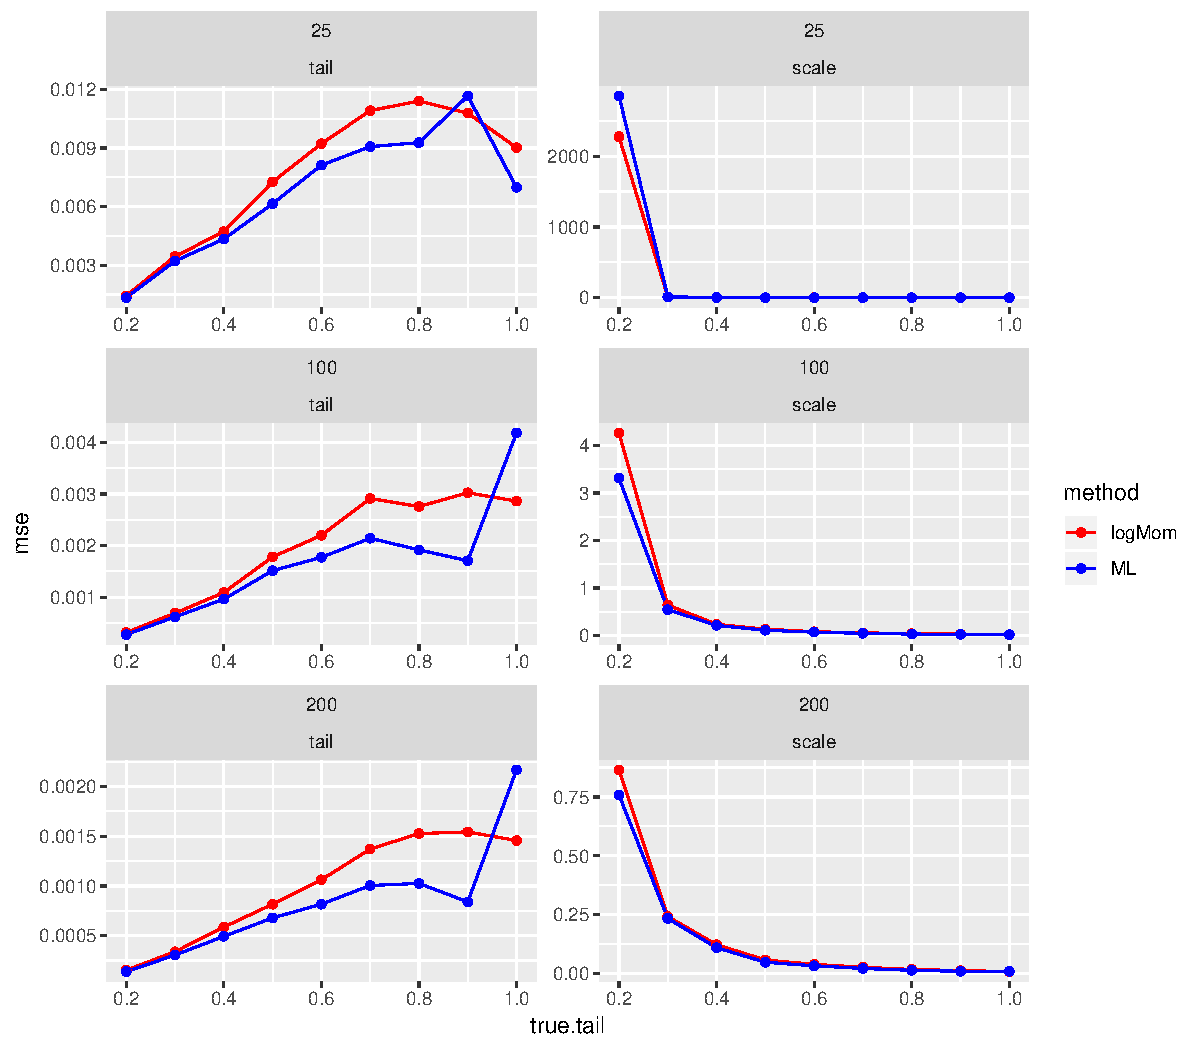
\includegraphics[width=0.9\linewidth]{article_springer_files/figure-latex/MSE-1} 

}

\caption{\label{fig:MSE} MSE for the estimation of tail (left column) and scale (right column) parameters via log-moment estimator and mle of a Mittag-Leffler sample with varying sample size n=25, 100, 200, varying tails on the x-axis and fixed scale equal to one.}\label{fig:MSE}
\end{figure}

Since the Mittag-Leffler distribution is heavy-tailed, many researchers
would intuitively give the highest importance to the tail behaviour of
the distribution. Of course, one can also use established tail exponent
estimators for the estimation of the parameter \(\beta\) such as the
Hill estimator (Hill 1975) based on the \(r+1\) upper order statistics
\begin{align}\label{eq:hill}
H_{r,n}=\left[ \frac{1}{r} \sum_{i=0}^{r} \log \frac{X_{(i)}}{X_{(r+1)}}\right]^{-1}, 
\end{align} where \(X_{(1)} \geq X_{(2)} \geq \ldots \geq X_{(n)}\)
denote the order statistics in decreasing order of a sequence
\(X_1,\ldots,X_n\). However, these methods are statistically less
efficient since they only use a portion of the information contained in
the data, as mentioned by Kozubowski (2001). Moreover, the hill
estimator requires a tuning parameter, denoted with \(r\) in
\eqref{eq:hill}. Additionaly, the estimator only performs reliably well
for distributions close to Pareto (see Resnick 1997). Figure
\ref{fig:Hillplots} shows Hill plots for Mittag-Leffler simulated data,
with varying sample sizes and tails. To deduce the correct tail
parameter estimates from these plots is virtually impossible. To
estimate the tail parameter of a Mittag-Leffler distribution with the
hill estimator, the sample size has to be much larger and one has to
choose a large tuning parameter \(r\). In case that only events above a
high threshold are recorded, even \(n=1000\) events are unrealistic.
Furthermore the Hill estimator of course completely fails if the
inter-arrival times are exponential distributed and not heavy-tailed. We
will comeback to the problems with the hill estimtator in Section
\ref{Simulationstudy}.

\begin{figure}

{\centering 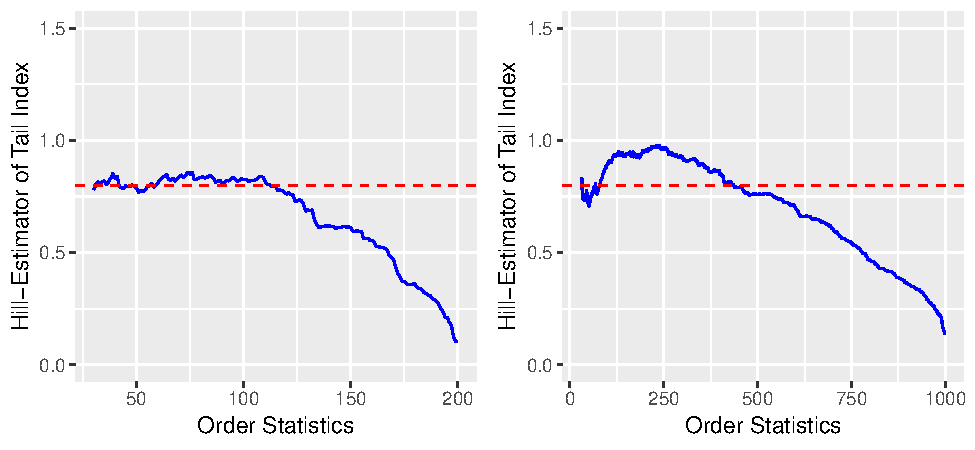
\includegraphics[width=0.9\linewidth]{article_springer_files/figure-latex/Hillplots-1} 

}

\caption{\label{fig:Hillplots} Hillplots for simulated Mittag-Leffler data with true tail 0.8 and sample size 200 (left) and 1000 (right), with number of upper order statics r on which the hill estimator is based on the x-axis. }\label{fig:Hillplots}
\end{figure}

Since the exponential distribution is nested in the Mittag-Leffler
family of distributions, a Likelihood-ratio Test (LRT) seems to be an
appropriate way to choose between a model with exponential and
Mittag-Leffler inter-exceedance times. Although the two models are
nested, the asymptotic distribution is not \(\chi^2_1\)-distributed, and
Wilk's Theorem does not hold: under \(H_0\), the parameter \(\beta\) of
Mittag-Leffler distribution is equal to \(1\), and hence lies on the
boundary of the parameter space \((0,1]\). Instead, a valid approach is
a bootstrapped Likelihood-ratio test (see e.g.~Davison, Hinkley, and
others 1997). Figure \ref{Fig:LRT} displays the (simulated) power for
the bootstrapped LRT for Mittag-Leffler distributions with varying tail
parameters based on 1000 simulation runs. As expected, the power
decreases for tail parameters close to one, since the Mittag-Leffler
distribution converges as \(\beta \uparrow 1\) to an exponential
distribution; it becomes hard to differentiate a Mittag-Lefller
distribution from an exponential.

\begin{figure}

{\centering 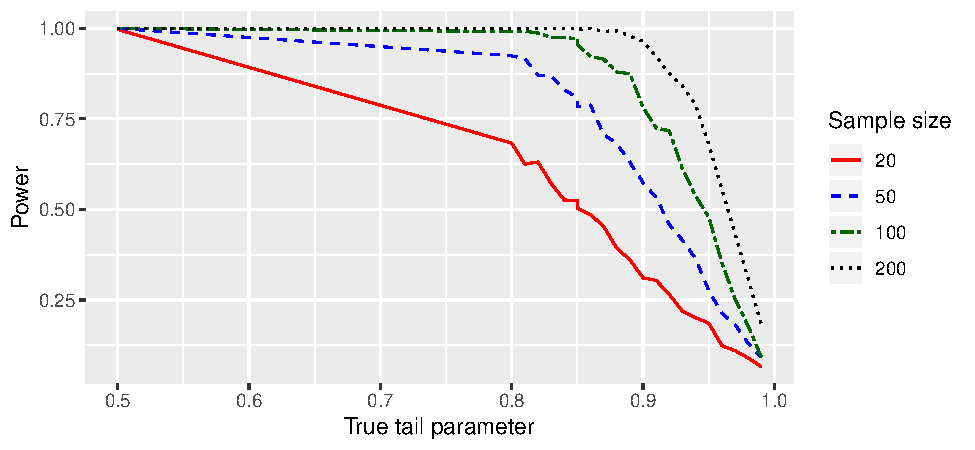
\includegraphics[width=0.9\linewidth]{article_springer_files/figure-latex/LRT_power-1} 

}

\caption{\label{Fig:LRT} Power for bootstrapped LRT for different sample sizes , varying tails and scale parameter equal to 1.}\label{fig:LRT_power}
\end{figure}

\hypertarget{inference-on-exceedance-times}{%
\section{Inference on Exceedance
times}\label{inference-on-exceedance-times}}

The Theorem in Section \ref{sec:scaling} implies that for a high
threshold \(\ell\) we may approximate the distribution of \(T(\ell)\)
with an \({\rm ML}(\beta, b(1/p))\) distribution, where the function
\(b(c)\) varies regularly at \(\infty\) with parameter \(1/\beta\).
Building on the POT (Peaks-Over-Threshold) method, we propose the
following estimation procedure for the distribution of inter-exceedance
time \(T(\ell)\):

\begin{enumerate}
\def\labelenumi{\arabic{enumi}.}
\item
  For a range of thresholds \(\ell\) near the largest order statistics,
  extract datasets of exceedance times \(\{T(\ell, i)\}_i\).
\item
  For each choice of threshold \(\ell\), fit a Mittag-Leffler
  distribution to the resulting dataset \(\{T(\ell, i)\}_i\). This
  results in the estimates \(\{\hat\beta(\ell)\}_\ell\) and
  \(\{\hat \sigma(\ell)\}_\ell\).
\item
  Plot \(\ell\) vs.~\(\hat \beta(\ell)\). As \(\ell\) increases towards
  \(x_R\), \(\hat \beta(\ell)\) \emph{stabilizes} around a constant
  \(\hat \beta\). Use \(\hat \beta\) as an estimate for the tail
  parameter \(\beta\) of the Mittag-Leffler distribution of exceedance
  times.
\item
  Approximate \(p \approx |\{k: J_k > \ell\}| / n\). Recall that
  \(b(c)\) is regularly varying with parameter \(1/\beta\), and hence
  has the representation \(b(c) = L(c) c^{1/\beta}\) for some slowly
  varying function \(L(c)\). Assuming that the variation of \(L(c)\) is
  negligible, we hence plot \(\ell\)
  vs.~\(p^{1/\hat \beta} \hat \sigma(\ell)\). Again as \(\ell\)
  increases towards \(x_R\), \(p^{1/\hat \beta} \hat \sigma(\ell)\) is
  expected to stabilize around a constant \(\hat \sigma_0\). We then use
  \(p^{-1/\hat \beta} \hat \sigma_0\) as an estimate of the scale
  parameter of the Mittag-Leffler distribution of exceedance times for
  the level \(\ell\).
\end{enumerate}

The above approach benefits from the following practical adjustments
(compare with Figure \ref{fig:flares}):

\begin{itemize}
\item
  We choose \(\ell\) from the order statistics, i.e.~\(\ell\) is the
  \(k\)-th largest of the observations \(X_j\), where \(k\) runs from
  \(k_\text{min}, k_\text{min} + 1, \ldots, k_\text{max}\). The datasets
  are then of length \(k-1\).
\item
  We use \(k\) rather than \(\ell\) for the horizontal axis of our
  plots.
\item
  In Step 4, rather than plotting \(p^{1/\hat \beta} \hat \sigma(\ell)\)
  we plot \(k^{1/\hat \beta} \hat \sigma(\ell)\). This changes
  \(\hat \sigma_0\) by the multiplicative constant \(n^{1/\hat \beta}\),
  but has the advantage that \(\hat \sigma_0\) does not change if one
  pre-processes the data by removing all observations below a certain
  threshold.
\end{itemize}

The estimates \(\hat \beta\) and \(\hat \sigma_0\) give an estimate of
the distribution of exceedance times, dependent on the threshold
\(\ell\): \begin{align*}
T(\ell) \sim {\rm ML}(\hat \beta, k^{-1/\hat \beta} \hat \sigma_0),
\end{align*} where \(\ell\) equals the \(k\)-th order statistic. For
quick estimates of the Mittag-Leffler parameters we have used the method
of log-transformed moments (Cahoy 2013). We have verified the validity
of our estimation algorithm via simulations, see Section
\ref{Simulationstudy}.

\hypertarget{Simulationstudy}{%
\section{Simulation study}\label{Simulationstudy}}

To test our inference method via stability plots, we have simulated
\(m=100\) times \(n=10000\) independent waiting time and magnitude pairs
\((W_k, J_k)\) for waiting times that follow

\begin{enumerate}
\def\labelenumi{(\roman{enumi})}
\item
  a stable distribution,
\item
  a Pareto distribution and
\item
  an exponential distribution.
\end{enumerate}

In order to have exact analytical values available for \(\beta\) and
\(\sigma_0\), a distribution for \(W_k\) needs to be chosen for which
\(b(n)\) from \eqref{eq:stability} is known. For (i) we choose
\(W_k \stackrel{d}{=} D\), where \(D\) is as in \eqref{eq:stability},
then due to the stability property we have the \emph{equality} of
distribution \(W_1 + \ldots + W_n \stackrel{d}{=} b(n) D\), for
\(b(n) = n^{1/\beta}\). Using the parametrisation of Samorodnitsky and
Taqqu (1994), a few lines of calculation (see e.g.~the vignette on
parametrisation in Gill and Straka 2017) show that \(D\) must have the
stable distribution \(S_\beta(\cos(\pi \beta/2)^{1/\beta}, +1, 0)\),
which is implemented in the R package \texttt{stabledist} by Wuertz,
Maechler, and members. (2016). By the Theorem, the distribution of
\(T(\ell)\) is approximately \[
{\rm ML}(\beta, p^{-1/\beta}) 
= {\rm ML}(\beta, k^{-1/\beta} n^{1/\beta}),
\] which means \(\sigma_0 = n^{1/\beta}\). In the Pareto example we
choose \(P(W>t)=Ct^{-\beta}\) with \(C=(1/\Gamma(1-\beta))^{1/\beta}\).
We have chosen \(\beta=0.8\) in the stable as well as in the Pareto
case. As third example we choose exponential distributed waiting times
with a rate of \(1\). Figure \ref{Fig:TailSimu} shows the stability
plots for the estimation of the tail parameter. Therefore,
\(\hat \beta(k)\) vs.~\(k\) is plotted for each of the \(m=100\)
simulation runs (grey thin lines). In the left column one can see the
estimates based on the log-moment estimator, the stability plots in the
middle are based on the maximum-likelihood estimator and on the right
hand on the hill estimator. Recall that \(k\) is the index of the order
statistics of \(J_k\) at which the threshold \(\ell\) is placed. Note,
that the hill estimator is here based on the waiting times, not on the
inter-exceedance times, hence the estimation is based on much more data.
If one would base the hill-estimation only on the inter-exceedance
times, the sample size would be too small and it would be impossible to
deduce an estimate for the tail parameter from the plots (compare Figure
\ref{fig:Hillplots}). The \(k\) on the \(x-\)axis is in the plots for
the hill estimator the \(r\) which defines on which upper orders stats
the hill estimator is based on (compare \eqref{eq:hill}). The bigger
sample size results in the middle in a lower bias. But, one can also
see, that there is much more variance between the stability plots for
the different simulation runs in case of the hill estimator compared to
the other two estimators. The black line is the mean value of the point
estimators for each \(k\) resp. \(r\). However, if one wants to get a
single estimate via such a stability plot, it would be much more
difficult to deduce it from a hill plot compared to the other two
estimators. In case that one has only thresholded data and hence a much
smaller simple size, the hill estimator gets useless (see Section
\ref{sec:ML}). Another advantage of the other estimators compared to the
hill estimator is, that in the case one has exponential waiting times,
the log-moment as well as the mle can detect this by getting an estimate
close to \(1\). The hill estimators is just a tail parameter estimator
for Pareto like tails and hence of course fails in case of exponential
distributed inter-exceedance times. Figure \ref{Fig:ScaleSimu} shows the
stability plots for the different estimators for the scale parameter.
Here of course only for the log-moment (on the right hand) and the mle
(on the left hand), since the hill estimator is just a tail parameter
estimate. Here again both estimators show good performance. The
stability plots in the mle case are a little bit closer to the true
value, except in the exponetial case. Therefore, the mle is much more
computational intensive.

\begin{figure}

{\centering 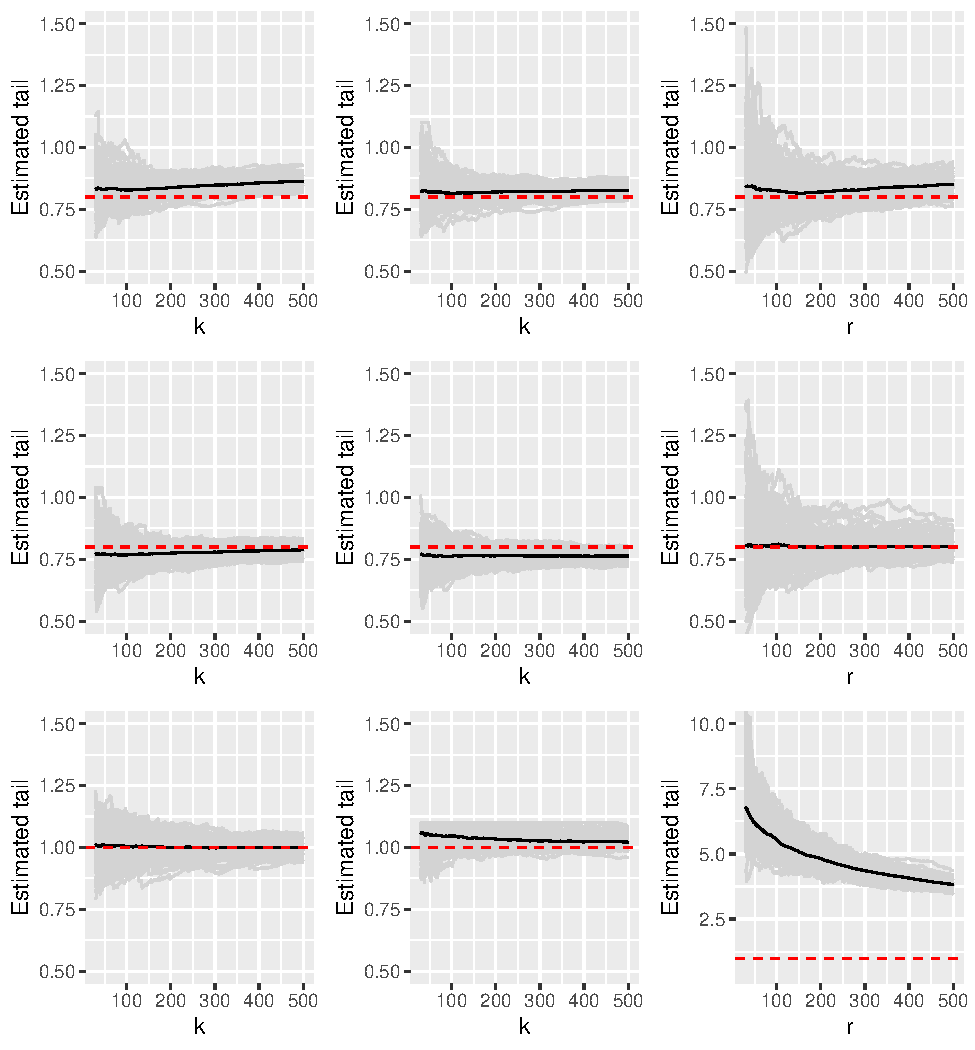
\includegraphics[width=1\linewidth]{article_springer_files/figure-latex/TailSimuplots-1} 

}

\caption{\label{Fig:TailSimu} Stability Plots for m=100 simulation runs for stable distributed waiting times with a tail parameter of 0.8 (top row), Pareto distributed waiting times with tail parameter 0.8 (middle row) and exponential distributed waiting times (lower row). Left column: log-moment estimator, middle column: MLE, right column: Hill estimator. The grey thin lines are the stability plots for the different simulation runs and the dark lines are their means. The red dotted line shows the true tail parameter. }\label{fig:TailSimuplots}
\end{figure}

\begin{figure}

{\centering 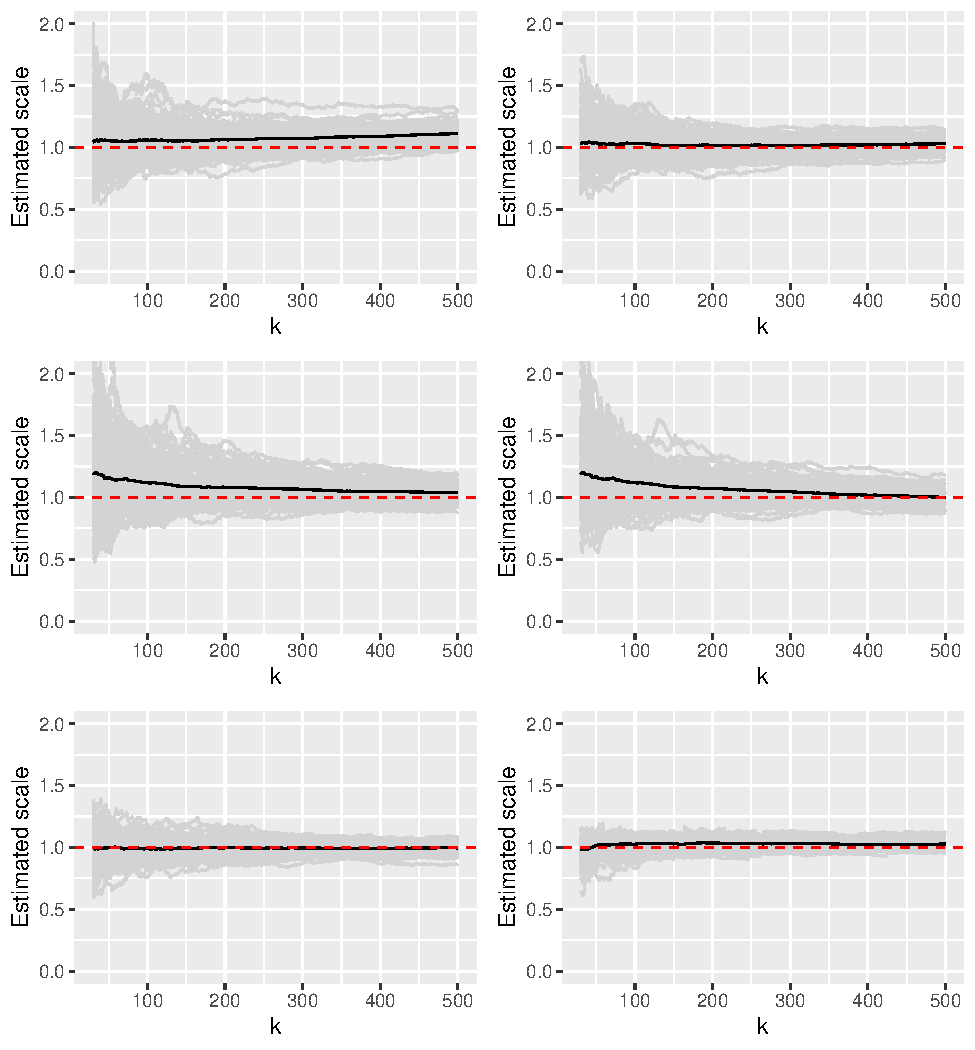
\includegraphics[width=0.9\linewidth]{article_springer_files/figure-latex/ScaleSimuplots-1} 

}

\caption{\label{Fig:ScaleSimu} Stability Plots for m=100 simulation runs for stable distributed waiting times with a tail parameter of 0.8 (top row), Pareto distributed waiting times with tail parameter 0.8 (middle row) and exponential distributed waiting times (lower row). Left column: log-moment estimator, right column: MLE. The grey thin lines are the stability plots for the different simulation runs and the dark lines are their means. The red dotted line shows the true tail parameter.}\label{fig:ScaleSimuplots}
\end{figure}

\hypertarget{data-example}{%
\section{Data example}\label{data-example}}

We now want to apply the proposed method to a real data example, the
solar flare data which was already mentioned in Section 1 and can be
seen in Figure \ref{fig:thresholdedBursty}. The data were extracted from
the ``complete Hard X Ray Burst Spectrometer event list'', a
comprehensive reference for all measurements of the Hard X Ray Burst
Spectrometer on NASA's Solar Maximum Mission from the time of launch on
Feb 14, 1980 to the end of the mission in Dec 1989. 12,772 events were
detected, with the ``vast majority being solar flares''. To assure
stationarity and due to missing values during the years 1983 and 1984,
we based our analysis just on the year 1982, in which 2,488 events
happened. The list includes the start time, peak time, duration, and
peak rate of each event. We have used ``start time'' as the variable for
event times, and ``peak rate'' as the variable for event magnitudes.

Before we apply the POT approach described in Section 5 to the solar
flare data, we first have to check if all model assumptions are
full-filled. The CTRE model is based on three main assumptions, which
are repeated below. For each assumption, we suggest one means of
checking if it holds:

\begin{description}
\item[i.i.d.:]
After removing the ``noise observations'' below the smallest threshold
\(\ell_0\), the pair sequence \((T(\ell_0, i), X(\ell_0,i))\) is i.i.d.
An indication if this is true is given by an auto-correlation plot for
the logarithms (to ensure finite moments) of the two time series.
\item[Uncoupled:]
Each \(T(\ell, i)\) is independent of each \(X(\ell, i)\). We propose an
empirical copula plot to check for any dependence.
\item[\({\rm ML}(\beta, \sigma)\) distribution of \(T(\ell, i)\):]
Apply a cutoff at the lowest threshold \(\ell_0\), extract the threshold
crossing times, and create a QQ Plot for the Mittag-Leffler
distribution. Use a log-moment estimate of the tail parameter for the
theoretical / population quantiles of the plot.
\end{description}

Figures \ref{fig:flare-diagnostics-1}, \ref{fig:flare-diagnostics-2} and
\ref{fig:flare-diagnostics-3} show the diagnostic plots for a minimum
threshold chosen at the 200th order statistic. There is some residual
autocorrelation for the sequence of threshold exceedance times that is
not accounted for by the CTRE model.

\begin{figure}
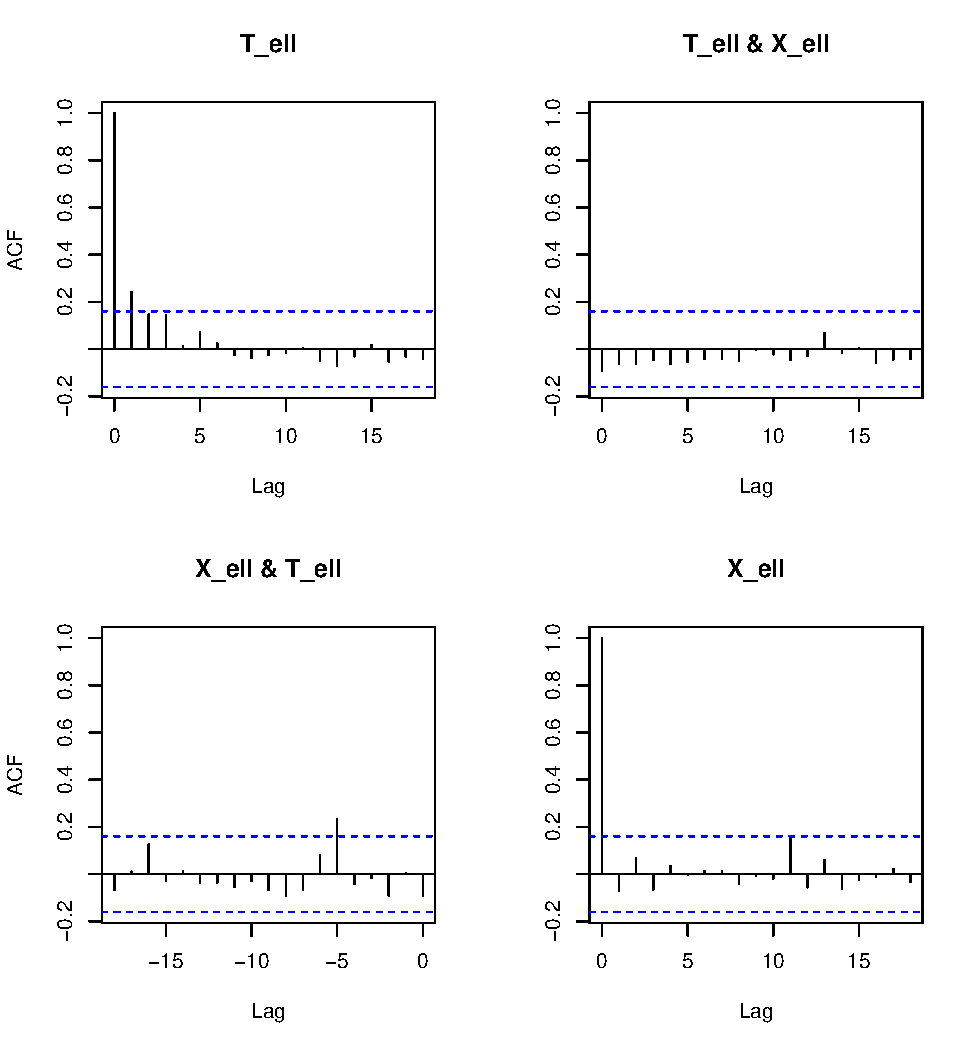
\includegraphics[width=\textwidth]{article_springer_files/figure-latex/flare-diagnostics-1-1} \caption{\label{fig:flare-diagnostics-1} Diagnostic plots for the solar flare data: auto-correlation function.}\label{fig:flare-diagnostics-1}
\end{figure}

\begin{figure}

{\centering 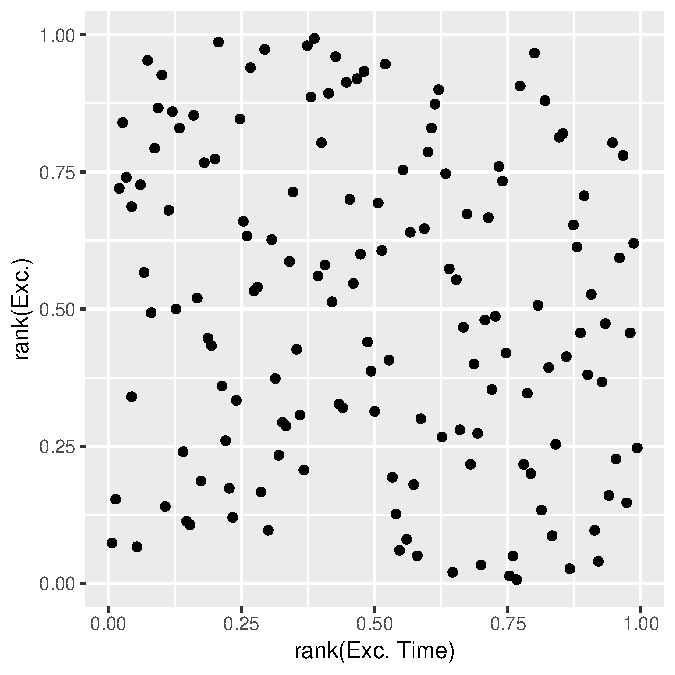
\includegraphics[width=0.7\linewidth]{article_springer_files/figure-latex/flare-diagnostics-2-1} 

}

\caption{\label{fig:flare-diagnostics-2} Diagnostic plots for the solar flare data: empirical copula.}\label{fig:flare-diagnostics-2}
\end{figure}

\begin{figure}

{\centering 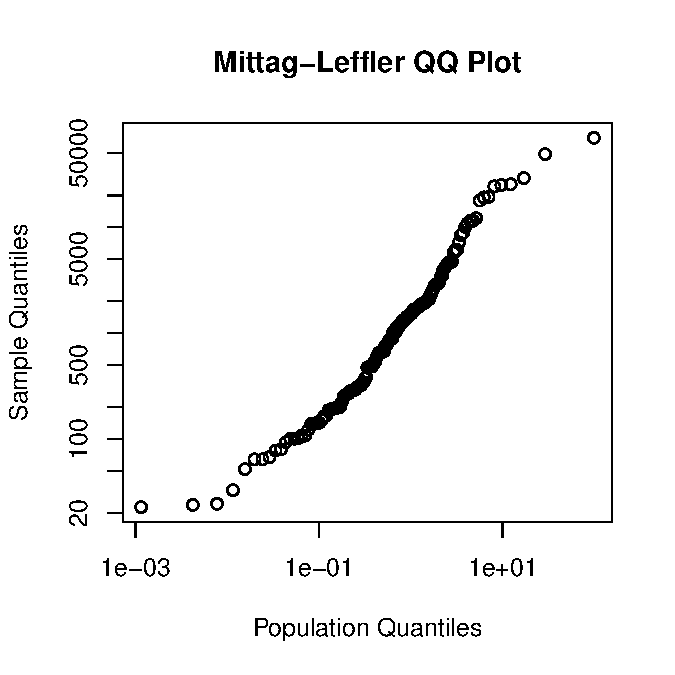
\includegraphics[width=0.7\linewidth]{article_springer_files/figure-latex/flare-diagnostics-3-1} 

}

\caption{\label{fig:flare-diagnostics-3} Diagnostic plots for the solar flare data: QQ Plot.}\label{fig:flare-diagnostics-3}
\end{figure}

Figure \ref{fig:flares} shows the stability plots for the solar flare
data, on the left for the tail parameter and on the right for the scale
parameter. Dotted lines show 95\% confidence intervals, which are
derived from the asymptotic normality of the log-moments estimators
(Cahoy 2013) and the \(\delta\)-method (Gill and Straka 2017), dashed
lines show the deduced values of \(\beta\) resp.~\(\sigma_0\). The
stability plot for the tail stabilizes nicely round about 0.85 (dashed
line), while it is a little bit harder to deduce an estimate for the
scale parameter. Howerever, the stability plot for the scale parameter
seems to stabilize round about \(3 \times 10^7\) (dashed line).

\begin{figure}
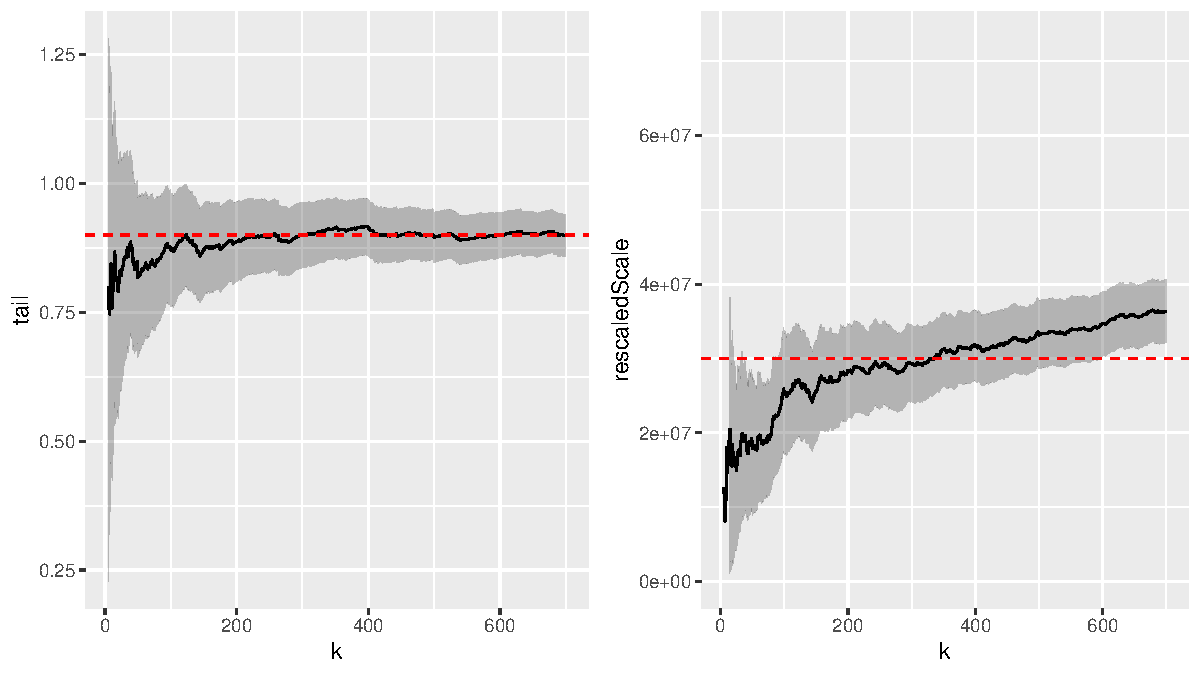
\includegraphics[width=\textwidth]{article_springer_files/figure-latex/solar-flare-tail-scale-1} \caption{\label{fig:flares} Stability plots for the tail and scale parameter of the Mittag-Leffler distribution of the Solar Flare dataset. Dotted horizontal lines are at $\beta = 0.85$ and $\sigma_0 = 3 \times 10^7$ seconds $\approx 0.95$ years.}\label{fig:solar-flare-tail-scale}
\end{figure}

The fit with a Mittag-Leffler distribution (\(\beta = 0.85\)) is good
(see Figure \ref{fig:flare-diagnostics-3}), though there are signs that
the power-law tail tapers off for very large inter-threshold crossing
times. There is no apparent dependence between threshold exceedance
times and event magnitudes seen in the copula plot (see Figure
\ref{fig:flare-diagnostics-2}). We also counduct a bootstrapped LRT for
the null hypothesis of exponential distributed inter-arrival times and
received a \(p\)-value of \(p<0.01\).

\hypertarget{predicting-the-time-of-the-next-threshold-crossing}{%
\section{Predicting the time of the next threshold
crossing}\label{predicting-the-time-of-the-next-threshold-crossing}}

According to Figure \ref{fig:flares}, for a threshold \(\ell\) at the
\(k\)-th order statistic, the fitted threshold exceedance time
distribution is \[
T(\ell) \sim {\rm ML}(\beta, k^{-1/\beta} \sigma_0), 
\] where \(\beta = 0.85\) and \(\sigma_0 = 3.0 \times 10^7 {\rm sec}\).
Unlike the exponential distribution, the Mittag-Leffler distribution is
not memoryless, and the probability density of the time \(t\) until the
next threshold crossing will depend on the time \(t_0\) elapsed since
the last threshold crossing. This density equals \[
p(t|\beta, \sigma_0, \ell, t_0) = \frac{f(t + t_0 | \beta, k^{-1/\beta} \sigma_0)}{\mathbf P[T_\ell > t_0]}
\] where \(f(\,\cdot\, | \beta, k^{-1/\beta} \sigma_0)\) is the
probability density of \({\rm ML}(\beta, k^{-1/\beta} \sigma_0)\). The
more time has passed without a threshold crossing, the more the
probability distribution shifts towards larger values for the next
crossing (see Figure \ref{fig:hazard}, left panel). The hazard rate \[
h(t) = \frac{f(t| \beta, k^{-1/\beta} \sigma_0))}{\int_t^\infty f(\tau| \beta, k^{-1/\beta} \sigma_0))\,d\tau}
\] represents the risk of a threshold crossing per unit time, and is a
decreasing function for the Mittag-Leffler distribution.

\begin{figure}
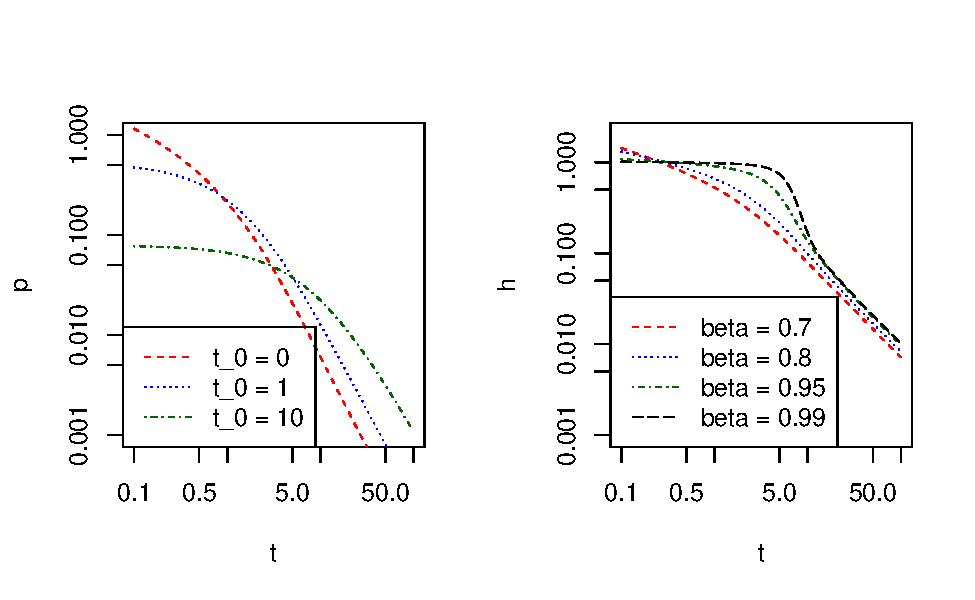
\includegraphics[width=\textwidth]{article_springer_files/figure-latex/hazard-1} \caption{\label{fig:hazard} Left: Conditional distribution of time until next threshold crossing, depending on elapsed time $t_0$ since last crossing ($\beta = 0.8$, $\sigma_0 = 1$). Right: Hazard rate depending on tail parameter $\beta$.}\label{fig:hazard}
\end{figure}

The closer \(\beta\) is to \(1\), the more the hazard rate mimics that
of an exponential distribution (a constant function, see Figure
\ref{fig:hazard}, right panel).

\hypertarget{discussion-conclusion}{%
\section{Discussion \& Conclusion}\label{discussion-conclusion}}

We have extended the POT (Peaks-over-Threshold) model, a mainstay of
extreme value theory, to ``bursty'' time series, which have been studied
intensively in statistical physics. Burstiness is characterized by
power-law waiting times between events, and we have shown that the
Mittag-Leffler distribution arises naturally as a scaling limit for the
inter-exceedance times of high thresholds. Moreover, we have derived the
following non-linear scaling behaviour: \(\sigma \sim p^{-1/\beta}\),
where \(\sigma\) is the scale parameter of the distribution of threshold
exceedance times, \(p\) is the fraction of magnitudes above the
threshold, and \(\beta\) the exponent of the power law. This
``anomalous'' scaling behaviour in the bursty setting entails two
phenomena:

\begin{enumerate}
\def\labelenumi{\roman{enumi})}
\item
  a heavy tail of the inter-arrival time distribution of threshold
  crossings (long rests), and
\item
  a high propensity for more threshold crossing events immediately after
  each threshold crossing event (bursts).
\end{enumerate}

The Mittag-Leffler distribution captures both phenomena, due to its
heavy tail as well as its stretched exponential (peaked) asymptotics for
small times. It generalizes the exponential distribution, and in the
solar flare data example, this generalization is warranted, because the
likelihood-ratio test is strongly significant.

When we introduced the CTRE model, we assumed that all events are i.i.d.
This assumption is likely sufficient but not necessary for our limit
theorem to hold. Moreover, any data below a (minimum) threshold
\(\ell_0\) is discarded for CTREs, and hence need not satisfy the i.i.d.
assumption.For the purposes of statistical inference, we merely require
that the inter-threshold-crossing times are i.i.d.

The bursty CTRE approach to model ``non-Poissonian'' threshold crossing
times should be contrasted with the (now standard) approach of clusters
of extremes, see e.g.~Ferro and Segers (2003). In this approach, i.i.d.
event sequences of magnitudes are generalized to stationary sequences of
event magnitudes (subject to a mixing condition). The two approaches are
fundamentally different: A clustering model assumes that each event
belongs to one particular (latent) group of events. For bursts, however,
the aim is to identify an underlying scale-free pattern in the event
dynamics, which is often characteristic of complex systems. It is an
interesting open problem to develop quality criteria, based e.g.~on
measures of surprise (Lee, Fan, and Sisson 2015), which guide an applied
statistician in the choice between a clustering and a CTRE approach for
a particular problem. Moreover, we believe it may be possible to unify
the two approaches by considering CTREs based on MRPs with a
\emph{stationary}, rather than i.i.d., sequence of magnitudes.

Finally, a purely scale-free pattern for event times may be too rigid as
an assumption for some bursty time series, because often the
heavy-tailed character of the inter-arrival time distribution does not
hold at all time scales; rather, it applies at short and intermediate
time scales, and is truncated (or tempered, reverting to an exponential
distribution) at very long time scales (see e.g.~Mark M. Meerschaert,
Roy, and Shao 2012; and Aban, Meerschaert, and Panorska 2006). In such
situations, a ``tempered'' Mittag-Leffler distribution may provide a
more realistic fit, which we aim to introduce in follow-up work.

\hypertarget{acknowledgements}{%
\section*{Acknowledgements}\label{acknowledgements}}
\addcontentsline{toc}{section}{Acknowledgements}

The authors would like to thank Prof.~Peter Scheffler for insights on
stochastic process limits for CTRMs, Prof.~Roland Fried for discussion
according the statistical methods and Gurtek Gill who helped create the
MittagLeffleR R-package.

\newpage

\hypertarget{references}{%
\section*{References}\label{references}}
\addcontentsline{toc}{section}{References}

\hypertarget{refs}{}
\leavevmode\hypertarget{ref-Aban06}{}%
Aban, Inmaculada B, Mark M Meerschaert, and Anna K Panorska. 2006.
``Parameter Estimation for the Truncated Pareto Distribution.'' \emph{J.
Am. Stat. Assoc.} 101 (473): 270--77.
\url{https://doi.org/10.1198/016214505000000411}.

\leavevmode\hypertarget{ref-Anderson1987}{}%
Anderson, Kevin K. 1987. ``Limit Theorems for General Shock Models with
Infinite Mean Intershock Times.'' \emph{J. Appl. Probab.} 24 (2):
449--56. \url{http://www.jstor.org/stable/3214268}.

\leavevmode\hypertarget{ref-Bagrow2013}{}%
Bagrow, James P., and Dirk Brockmann. 2013. ``Natural emergence of
clusters and bursts in network evolution.'' \emph{Phys. Rev. X} 3 (2):
1--6. \url{https://doi.org/10.1103/PhysRevX.3.021016}.

\leavevmode\hypertarget{ref-Barabasi2005}{}%
Barabási, Albert László. 2005. ``The origin of bursts and heavy tails in
human dynamics.'' \emph{Nature} 435 (May): 207--11.
\url{https://doi.org/10.1038/nature03459}.

\leavevmode\hypertarget{ref-Basrak2014}{}%
Basrak, Bojan, and Drago Špoljarić. 2015. ``Extremes of random variables
observed in renewal times.'' \emph{Stat. Probab. Lett.} 97: 216--21.
\url{https://doi.org/10.1016/j.spl.2014.11.025}.

\leavevmode\hypertarget{ref-beirlantBook}{}%
Beirlant, Jan, Yuri Goegebeur, Johan Segers, and Jozef Teugels. 2006.
\emph{Statistics of extremes: theory and applications}. John Wiley \&
Sons.

\leavevmode\hypertarget{ref-Benson2007}{}%
Benson, David A, Rina Schumer, and Mark M Meerschaert. 2007.
``Recurrence of extreme events with power-law interarrival times.''
\emph{Geophys. Res. Lett.} 34 (l16404): DOI:10.1029/2007GL030767.
\url{https://doi.org/10.1029/2007GL030767}.

\leavevmode\hypertarget{ref-Cahoy2013}{}%
Cahoy, Dexter O. 2013. ``Estimation of Mittag-Leffler Parameters.''
\emph{Commun. Stat. - Simul. Comput.} 42 (2): 303--15.
\url{https://doi.org/10.1080/03610918.2011.640094}.

\leavevmode\hypertarget{ref-Cahoy2010}{}%
Cahoy, Dexter O, Vladimir V. Uchaikin, and Wojbor A. Woyczynski. 2010.
``Parameter estimation for fractional Poisson processes.'' \emph{J.
Stat. Plan. Inference} 140 (11): 3106--20.
\url{https://doi.org/10.1016/j.jspi.2010.04.016}.

\leavevmode\hypertarget{ref-ColesBook}{}%
Coles, S. 2001. \emph{An Introduction to Statistical Modelling of
Extreme Values}. London: Springer-Verlag.

\leavevmode\hypertarget{ref-davison1997bootstrap}{}%
Davison, Anthony Christopher, David Victor Hinkley, and others. 1997.
\emph{Bootstrap Methods and Their Application}. Vol. 1. Cambridge
university press.

\leavevmode\hypertarget{ref-HXRBS}{}%
Dennis, Brian R, L E Orwig, G S Kennard, G J Labow, R A Schwartz, A R
Shaver, and A K Tolbert. 1991. ``The complete Hard X Ray Burst
Spectrometer event list, 1980-1989.''
\url{https://umbra.nascom.nasa.gov/smm/hxrbs.html}.

\leavevmode\hypertarget{ref-Esary1973}{}%
Esary, J. D., and A. W. Marshall. 1973. ``Shock Models and Wear
Processes.'' \url{https://doi.org/10.1214/aop/1176996891}.

\leavevmode\hypertarget{ref-ferro2003inference}{}%
Ferro, Christopher AT, and Johan Segers. 2003. ``Inference for Clusters
of Extreme Values.'' \emph{Journal of the Royal Statistical Society:
Series B (Statistical Methodology)} 65 (2): 545--56.

\leavevmode\hypertarget{ref-MittagLeffleR}{}%
Gill, Gurtek, and Peter Straka. 2017. \emph{MittagLeffleR: Using the
Mittag-Leffler Distributions in R}.
\url{https://strakaps.github.io/MittagLeffleR/}.

\leavevmode\hypertarget{ref-Gut1999}{}%
Gut, Allan, and Jürg Hüsler. 1999. ``Extreme Shock Models.''
\emph{Extremes}, no. 1983: 295--307.
\url{http://link.springer.com/article/10.1023/A:1009959004020}.

\leavevmode\hypertarget{ref-Haubold11}{}%
Haubold, H. J., A. M. Mathai, and R. K. Saxena. 2011. ``Mittag-Leffler
Functions and Their Applications.'' \emph{J. Appl. Math.} 2011: 1--51.
\url{https://doi.org/10.1155/2011/298628}.

\leavevmode\hypertarget{ref-hawkes1971point}{}%
Hawkes, Alan G. 1971. ``Point spectra of some mutually exciting point
processes.'' \emph{J. R. Stat. Soc. Ser. B Stat. Methodol.}, 438--43.

\leavevmode\hypertarget{ref-hees2017coupled}{}%
Hees, Katharina, and Hans-Peter Scheffler. 2018a. ``Coupled Continuous
Time Random Maxima.'' \emph{Extremes} 21 (2).

\leavevmode\hypertarget{ref-hees2016joint}{}%
---------. 2018b. ``On Joint Sum/Max Stability and Sum/Max Domains of
Attraction.'' \emph{Probability and Mathematical Statistics} 38 (1).

\leavevmode\hypertarget{ref-hill1975simple}{}%
Hill, Bruce M. 1975. ``A Simple General Approach to Inference About the
Tail of a Distribution.'' \emph{The Annals of Statistics}, 1163--74.

\leavevmode\hypertarget{ref-Karsai2012}{}%
Karsai, Márton, Kimmo Kaski, Albert László Barabási, and János Kertész.
2012. ``Universal features of correlated bursty behaviour.'' \emph{Sci.
Rep.} 2. \url{https://doi.org/10.1038/srep00397}.

\leavevmode\hypertarget{ref-Karsai2011}{}%
Karsai, Márton, M. Kivelä, R. K. Pan, K. Kaski, J. Kertész, Albert
László Barabási, and J. Saramäki. 2011. ``Small but slow world: How
network topology and burstiness slow down spreading.'' \emph{Phys. Rev.
E - Stat. Nonlinear, Soft Matter Phys.} 83: 1--4.
\url{https://doi.org/10.1103/PhysRevE.83.025102}.

\leavevmode\hypertarget{ref-kozubowski2001}{}%
Kozubowski, Tomasz J. 2001. ``Fractional Moment Estimation of Linnik and
Mittag-Leffler Parameters.'' \emph{Mathematical and Computer Modelling}
34 (9-11): 1023--35.

\leavevmode\hypertarget{ref-Laskin2003}{}%
Laskin, Nick. 2003. ``Fractional Poisson process.'' \emph{Commun.
Nonlinear Sci. Numer. Simul.} 8 (3-4): 201--13.
\url{https://doi.org/10.1016/S1007-5704(03)00037-6}.

\leavevmode\hypertarget{ref-Lee15}{}%
Lee, J., Y. Fan, and S. A. Sisson. 2015. ``Bayesian threshold selection
for extremal models using measures of surprise.'' \emph{Comput. Stat.
Data Anal.} 85: 84--99.
\url{https://doi.org/10.1016/j.csda.2014.12.004}.

\leavevmode\hypertarget{ref-Meerschaert2010b}{}%
Meerschaert, Mark M, Erkan Nane, and P. Vellaisamy. 2011. ``The
fractional Poisson process and the inverse stable subordinator.''
\emph{Electron. J. Probab.} 16: 1600--1620.
\url{https://doi.org/10.1214/EJP.v16-920}.

\leavevmode\hypertarget{ref-MeerschaertRoyQin}{}%
Meerschaert, Mark M., Parthanil Roy, and Qin Shao. 2012. ``Parameter
estimation for exponentially tempered power law distributions.''
\emph{Commun. Stat. - Theory Methods} 41 (10): 1839--56.
\url{https://doi.org/10.1080/03610926.2011.552828}.

\leavevmode\hypertarget{ref-MeerschaertSikorskii}{}%
Meerschaert, Mark M, and Alla Sikorskii. 2012. \emph{Stochastic Models
for Fractional Calculus}. Vol. 43. Walter de Gruyter.

\leavevmode\hypertarget{ref-MeerschaertStoev08}{}%
Meerschaert, Mark M, and Stilian A Stoev. 2008. ``Extremal limit
theorems for observations separated by random power law waiting times.''
\emph{J. Stat. Plan. Inference} 139 (7): 2175--88.
\url{https://doi.org/10.1016/j.jspi.2008.10.005}.

\leavevmode\hypertarget{ref-Min2010}{}%
Min, Byungjoon, K. I. Goh, and Alexei Vazquez. 2011. ``Spreading
dynamics following bursty human activity patterns.'' \emph{Phys. Rev. E
- Stat. Nonlinear, Soft Matter Phys.} 83 (3): 2--5.
\url{https://doi.org/10.1103/PhysRevE.83.036102}.

\leavevmode\hypertarget{ref-Oliveira2005}{}%
Oliveira, J, and Albert László Barabási. 2005. ``Darwin and Einstein
correspondence patterns.'' \emph{Nature} 437 (October): 1251.
\url{https://doi.org/10.0138/4371251a}.

\leavevmode\hypertarget{ref-Omi2011}{}%
Omi, Takahiro, and Shigeru Shinomoto. 2011. ``Optimizing Time Histograms
for Non-Poissonian Spike Trains.'' \emph{Neural Comput.} 23 (12):
3125--44. \url{https://doi.org/10.1162/NECO_a_00213}.

\leavevmode\hypertarget{ref-Hsing88}{}%
``On the Exceedance Point Process for a Stationary Sequence.'' 1988 78:
97--112.

\leavevmode\hypertarget{ref-R}{}%
R Core Team. 2018. \emph{R: A Language and Environment for Statistical
Computing}. Vienna, Austria: R Foundation for Statistical Computing.
\url{https://www.R-project.org/}.

\leavevmode\hypertarget{ref-Resnick97}{}%
Resnick, Sidney I. 1997. ``Heavy tail modeling and teletraffic data.''
\emph{Ann. Stat.} 25 (5): 1805--49.
\url{https://doi.org/10.1214/aos/1069362376}.

\leavevmode\hypertarget{ref-SamorodnitskyTaqqu}{}%
Samorodnitsky, Gennady, and Murad S Taqqu. 1994. \emph{Stable
Non-Gaussian Random Processes: Stochastic Models with Infinite
Variance}. Stochastic Modeling. London: Chapman Hall.

\leavevmode\hypertarget{ref-Sumita1983}{}%
Shanthikumar, J. George, and Ushio Sumita. 1983. ``General shock models
associated with correlated renewal sequences.'' \emph{J. Appl. Probab.}
20 (3): 600--614. \url{http://www.jstor.org/stable/3213896}.

\leavevmode\hypertarget{ref-Sumita1984}{}%
---------. 1984. ``Distribution Properties of the System Failure Time in
a General Shock Model.'' \emph{Adv. Appl. Probab.} 16 (2): 363--77.
\url{http://www.jstor.org/stable/1427074}.

\leavevmode\hypertarget{ref-Sumita1985}{}%
---------. 1985. ``A class of correlated cumulative shock models.''
\emph{Adv. Appl. Probab.} 17 (2): 347--66.
\url{http://www.jstor.org/stable/1427145}.

\leavevmode\hypertarget{ref-Silvestrov2002a}{}%
Silvestrov, Dmitrii S. 2002. \emph{Limit Theorems for Randomly Stopped
Stochastic Processes}. Springer (Berlin, Heidelberg).

\leavevmode\hypertarget{ref-ST04}{}%
Silvestrov, Dmitrii S, and Jozef L. Teugels. 2004. ``Limit theorems for
mixed max-sum processes with renewal stopping.'' \emph{Ann. Appl.
Probab.} 14 (4): 1838--68.
\url{https://doi.org/10.1214/105051604000000215}.

\leavevmode\hypertarget{ref-Vajna2013}{}%
Vajna, Szabolcs, Bálint Tóth, and János Kertész. 2013. ``Modelling
bursty time series.'' \emph{New J. Phys.} 15 (10): 103023.
\url{https://doi.org/10.1088/1367-2630/15/10/103023}.

\leavevmode\hypertarget{ref-Vasquez2006}{}%
Vasquez, a, J G Oliveira, Z Dezso, K-I Goh, I Kondor, and Albert László
Barabási. 2006. ``Modeling bursts and heavy tails in human dynamics.''
\emph{Phys. Rev. E} 73: 361271--3612718.
\url{http://arxiv.org/abs/0510117v1}.

\leavevmode\hypertarget{ref-Vazquez2007}{}%
Vazquez, Alexei, Balázs Rácz, András Lukács, and Albert László Barabási.
2007. ``Impact of non-poissonian activity patterns on spreading
processes.'' \emph{Phys. Rev. Lett.} 98 (APRIL): 1--4.
\url{https://doi.org/10.1103/PhysRevLett.98.158702}.

\leavevmode\hypertarget{ref-stabledist}{}%
Wuertz, Diethelm, Martin Maechler, and Rmetrics core team members. 2016.
\emph{Stabledist: Stable Distribution Functions}.
\url{https://CRAN.R-project.org/package=stabledist}.


\end{document}


